% June 2015 (TOC contents linked in blue in pdf file)
%This template was prepared by Dorothea F. Brosius of the
%Institute for Electronics and Applied Physics, University of Maryland, College Park, MD
%The template was last updated in June 2015
%Thesis Main Page used with thesis.sty based on the
%University of Maryland Electronic Thesis and Dissertation (ETD) Style Guide (2014)

%The YourInformation file was created by Freja Nordsiek, 2014.
%Code for linking the TOC titles to the text in the pdf file was created by Freja Nordsiek, 2014.

%Code clean-up and addition of glossaries by Patrick Stanley, 2017.
%Assumed printing to pdf and extra sections not needed (such as preface and forward)

\documentclass[12pt]{thesis}

%some packages may not be needed depending on your use
\usepackage{titlesec}
   \titleformat{\chapter}
      {\normalfont\large}{Chapter \thechapter:}{1em}{}
\usepackage{lipsum} %Remove before final draft, used to generate filler text
\usepackage{graphicx}
  \graphicspath{ {images/} } %defining where images go here so I don't have to every time
\usepackage{cite}
\usepackage{lscape}
\usepackage{indentfirst}
\usepackage{latexsym}
\usepackage{multirow}
\usepackage{tabls}
\usepackage{wrapfig}
\usepackage{longtable}
\usepackage{supertabular}
%\usepackage{subeqn} %removed to fix error with glossaries package
\usepackage{subfigure}
\usepackage{microtype}
\usepackage[bookmarks, colorlinks=true, plainpages=false, pdfpagelabels, citecolor=blue, urlcolor=blue, filecolor=blue, linkcolor=blue]{hyperref} %creates hyperlinks to various sections in pdf
\usepackage[toc, nonumberlist]{glossaries} %needs to be after hyperref

\newcommand{\tbsp}{\rule{0pt}{18pt}} %used to get a vertical distance after \hline
\renewcommand{\baselinestretch}{2}
\setlength{\textwidth}{5.9in}
\setlength{\textheight}{9in}
\setlength{\topmargin}{-.50in}
\setlength{\oddsidemargin}{.55in}
\setlength{\parindent}{.4in}
\pagestyle{empty}


\setacronymstyle{long-short} %first use of acronym gives full name
\glsdisablehyper %turns off hyperlinking
\loadglsentries{definitions} %defines file with all entries
\renewcommand{\glossarysection}[2][]{} %Hides glossary title so it can be named manually
\makeglossaries


\begin{document}
\hypersetup{pageanchor=false} %Fixes hyperref error with unnumbered title pages
% !TEX root = ../mainthesis.tex

%Abstract Page

\hbox{\ }

\renewcommand{\baselinestretch}{1}
\small \normalsize

\begin{center}
\large{{ABSTRACT}}

\vspace{3em}

\end{center}
\hspace{-.15in}
\begin{tabular}{ll}
Title of dissertation:    & {\large  EVALUATION OF STRENGTH AND  }\\
&				      {\large  RELIABILITY OF SOLID-OXIDE FUEL } \\
&				      {\large  CELLS AT OPERATING CONDITIONS} \\
\ \\
&                          {\large  Patrick Stanley, Doctor of Philosophy, 2018} \\
\ \\
Dissertation directed by: & {\large  Professor Eric D. Wachsman} \\
&  				{\large	 Materials Science and Engineering } \\
\end{tabular}

\vspace{3em}

\renewcommand{\baselinestretch}{2}
\large \normalsize

\lipsum[1-4] %Replace with actual text
 %(must be first, required, non-numbered)
% !TEX root = ../mainthesis.tex

%Titlepage

\thispagestyle{empty}
\hbox{\ }
\vspace{1in}
\renewcommand{\baselinestretch}{1}
\small\normalsize
\begin{center}

\large{{EVALUATION OF STRENGTH AND RELIABILITY OF SOLID-OXIDE FUEL CELLS AT OPERATING CONDITIONS}}\\
\ \\
\ \\
\large{by} \\
\ \\
\large{Patrick Owen Stanley}%Your full name as it appears in University records.
\ \\
\ \\
\ \\
\ \\
\normalsize
Dissertation submitted to the Faculty of the Graduate School of the \\
University of Maryland, College Park in partial fulfillment \\
of the requirements for the degree of \\
Doctor of Philosophy \\
2018
\end{center}

\vspace{7.5em}

\noindent Advisory Committee: \\
Professor Eric D. Wachsman: \textit{Advisor, Chair} \\
Professor Abhijit Dasgupta: \textit{Dean's Representative} \\
Professor Isabel K. Lloyd \\
Professor Lourdes Salamanca-Riba \\
Professor Sreeramamurthy Ankem
 %(must follow Abstract, required, non-numbered)
% !TEX root = ../mainthesis.tex

%Copyright

\thispagestyle{empty}
\hbox{\ }

\vfill
\renewcommand{\baselinestretch}{1}
\small\normalsize

\vspace{-.65in}

\begin{center}
\large{\copyright \hbox{ }Copyright by\\
Patrick Owen Stanley  %Type your name as it appears in University records
\\
2018}
\end{center}

\vfill
 %(highly recommended, non-numbered)
\hypersetup{pageanchor=true}

%Pages from this point start at lower-case Roman number ii)
\pagestyle{plain}
\pagenumbering{roman}
\setcounter{page}{2}

\addcontentsline{toc}{chapter}{Dedication}
% !TEX root = mainthesis.tex

%Dedication

\renewcommand{\baselinestretch}{2}
\small\normalsize
\hbox{\ }

\vspace{-.65in}

\begin{center}
\large{Dedication}
\end{center}

\noindent I dedicate this work to my wife who has supported and encouraged me throughout.
 %(if present, lower-case Roman)

\addcontentsline{toc}{chapter}{Acknowledgements}
% !TEX root = mainthesis.tex

%Acknowledgments

\renewcommand{\baselinestretch}{2}
\small\normalsize
\hbox{\ }

\vspace{-.65in}

\begin{center}
\large{Acknowledgments}
\end{center}

\vspace{1ex}

\lipsum[2-4] %replace with actual text
 %(if present, lower-case Roman)

\renewcommand{\baselinestretch}{1}
\small\normalsize

\tableofcontents %(required, lower-case Roman)

\newpage
\listoftables %(if present, lower-case Roman)

\newpage
\listoffigures %(if present, lower-case Roman)

\newpage
\addcontentsline{toc}{chapter}{List of Abbreviations and Symbols} %Manually put in ToC
\renewcommand{\baselinestretch}{1}
\small\normalsize
\hbox{\ }

\begin{center}
\large{List of Abbreviations and Symbols} %Manually create centered title
\end{center}

\vspace{3pt}

\printglossary


\newpage
\setlength{\parskip}{0em}
\renewcommand{\baselinestretch}{2}
\small\normalsize

%Pages from this point start at Arabic numeral 1
\setcounter{page}{1}
\pagenumbering{arabic}
% !TEX root = mainthesis.tex

%Chapter 1

%\renewcommand{\thechapter}{1}

\chapter{Introduction}

\section{Solid-Oxide Fuel Cells}

This piece will talk about \glspl{sofc}. This is mostly because I work on \glspl{sofc}. %Example of using glossaries package
For a picture of an \gls{sofc} see Figure \ref{image:sofc}.
\begin{figure}[h]
  \centering
  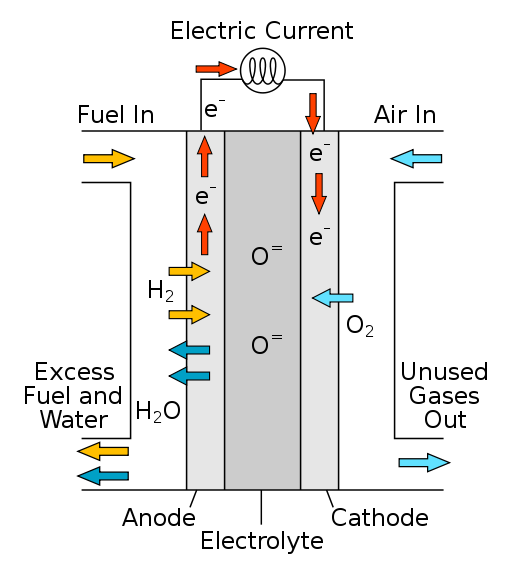
\includegraphics[width=0.5\textwidth]{sofc.png}
  \caption{Diagram showing flow of materials in the operation of a SOFC.\cite{Sakurambo}}
  \label{image:sofc}
\end{figure}

\lipsum\cite{Wang2006a} %Replace with actual text plus example of citation

% !TEX root = mainthesis.tex

%Chapter 2

%\renewcommand{\thechapter}{2}

\chapter{Experimental Procedures}

\section{Overview}

\lipsum%Replace with actual text

% !TEX root = ../mainthesis.tex

%Chapter 3

%\renewcommand{\thechapter}{3}

\chapter{Development of Testing Apparatus}

\section{Overview}

\lipsum %Replace with actual text


\appendix
\titleformat{\chapter}
      {\normalfont\large}{Appendix \thechapter:}{1em}{}
% !TEX root = ../mainthesis.tex

%Appendix -- January 2015
%\appendix
%\renewcommand{\thechapter}{A}
%\renewcommand{\chaptername}{Appendix}

\chapter{Weibull Statistics}

\lipsum %Replace with actual text

% !TEX root = mainthesis.tex

%Appendix -- January 2015
%\appendix
%\renewcommand{\thechapter}{B}
%\renewcommand{\chaptername}{Appendix}

\chapter{Code}

\lipsum %Replace with actual text


\renewcommand{\baselinestretch}{1}
\small\normalsize

%Assuming you are using BibTeX
\newpage
\bibliographystyle{unsrt}
\bibliography{Bibliography}

\end{document}
